\documentclass{beamer}

\usetheme{CambridgeUS}
\usepackage{float}
\usepackage{caption}
\usepackage{graphicx}
\title{Assignment 5(CBSE 12 Example 35)} 
\author{Akhila Kumbha,CS21BTECH11031}
\date{\today}
\logo{\large \LaTeX{}}


\providecommand{\brak}[1]{\ensuremath{\left(#1\right)}}
\newcommand{\myvec}[1]{\ensuremath{\begin{pmatrix}#1\end{pmatrix}}}
\providecommand{\pr}[1]{\ensuremath{\Pr\left(#1\right)}}
\begin{document}


\begin{frame}
    \titlepage 
\end{frame}

\logo{}

\begin{frame}{Outline}
    \tableofcontents
\end{frame}


\section{Question}
\begin{frame}{Question}

The probability of a shooter hitting a target is $\frac{3}{4}$. How many minimum
number of times must he/she fire so that the probability of hitting the target at least
once is more than 0.99?\\

\end{frame}


\section{Solution}
\begin{frame}{Solution}
Let the shooter fire $n$ times. Obviously, $n$ fires are $n$ Bernoulli trials.\\
In each trial,\\
p = probability of hitting the target =$\frac{3}{4}$ \\
q = probability of not hitting the target =$\frac{1}{4}$.\\

Let $X$ be the random variable whose probability distribution is B\brak{n,\frac{3}{4}}.\\
We know that,
\begin{align}
\pr{X=k}&=\myvec{n \\ k}q^{n-k}p^k ,k=0,1,2,\dots n\\
    &=\myvec{n \\ k}\brak{\frac{1}{4}}^{n-k}\brak{\frac{3}{4}}^k\\
    &=\myvec{n \\ k}\frac{3^k}{4^n}
\end{align}
\end{frame} 

\begin{frame}{Solution(contd)}
  Now, given that,
\begin{align}
\pr{\text {hitting the target at least once}} > 0.99\\
\implies \pr{X\geq 1} > 0.99\\
\implies 1-\pr{X=0} > 0.99\\
\implies 1-\myvec{n \\ 0}\frac{3^0}{4^n} > 0.99\\
\implies \myvec{n \\ 0}\frac{1}{4^n} < 0.01\\
\implies \frac{1}{4^n} < 0.01\\
\implies 4^n > 100
\end{align}
The minimum value of $n$ to satisfy the above inequality is 4.\\
Thus, the shooter must fire 4 times.   
\end{frame}

\subsection{PMF}
\begin{frame}{PMF}
\begin{figure}[H]
    \centering
    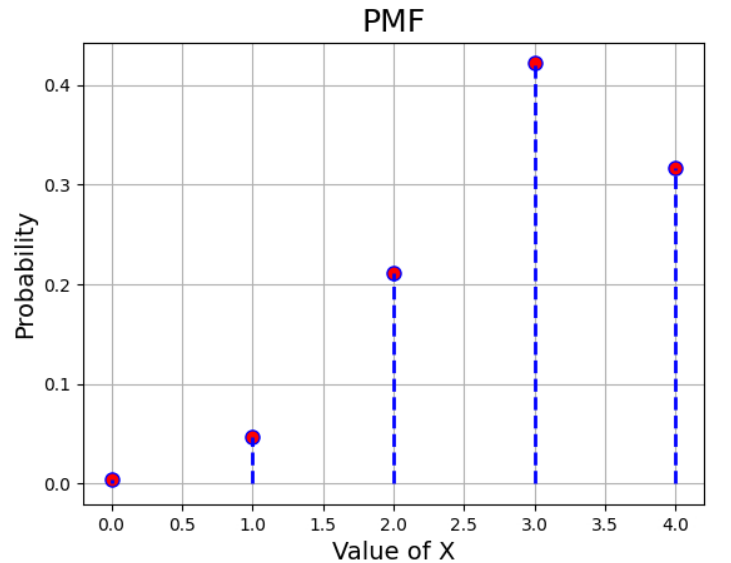
\includegraphics[width=7cm,height=6cm]{plot5.png}
    \captionsetup{justification=centering,margin=1cm}
    \caption{Plot of the PMF}
    \label{fig:plot5}
\end{figure}
\end{frame}


\end{document}